\documentclass[10pt,a4paper,tikz,border=20pt]{standalone}
\usepackage[utf8]{inputenc}
\usepackage[T1]{fontenc}
\usepackage{amsmath}
%\usepackage{amsfonts}
\usepackage{amssymb}
\usepackage{mathtools}
\DeclarePairedDelimiter\abs{\lvert}{\rvert}
\usepackage{tikz}
\usetikzlibrary{shapes,arrows,shapes.misc}
\usetikzlibrary{positioning}
\usepackage{gitinfo2}
\usepackage{graphicx}
\renewcommand{\gitMark}{Branch:\,\gitBranch\,@\,\gitAbbrevHash{}; Author:\,\gitAuthorName; Date:\,\gitAuthorIsoDate~\textbullet{}}
\makeatletter
\AddToShipoutPictureBG{%
	\AtPageLowerLeft{%
		\kern2.6cm
		\raisebox{\dimexpr.5\paperheight-.8\height}
		{\rotatebox{90}{\gitMarkFormat\gitMarkPref{} \textbullet{} \gitMark}}%
	}%
}%
\makeatother
\newcommand{\sempvert}{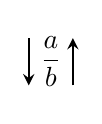
\begin{tikzpicture}[thick]
		\def\y{2.8mm}
		\def\x{2.8mm}
		\def\h{3.0mm}
		\def\dist{12mm}%1cm
		\node at (0,0) {$\displaystyle \frac{a}{b}$};
	%	\node at (\dist,0) {$\displaystyle \frac{c}{d}$};
		%\node at (2.5*\dist,0) {$a\cdot d=b\cdot c$};
		% collegamento termini
		\draw[-stealth] (-\y, \h)--(-\y,-\h); 
		\draw[-stealth] (\x,-\h)--(\x, \h);
	\end{tikzpicture}%
}
%\renewcommand{\gitMarkFormat}{\color{blue}\sffamily\bfseries}
\begin{document}
\tikzset{
	decision/.style={diamond, draw, %fill=blue!20,
		text width=4.5em, text badly centered, 
		node distance=3.5cm, inner sep=0pt
	},
	block/.style={rectangle, draw, %fill=blue!20,
		text width=15em, text centered, 
		node distance=2.5cm,
		%rounded corners, 
		minimum height=3em
	},
	loop/.style={chamfered rectangle,chamfered rectangle 	xsep=2cm, draw, %fill=blue!20,
		text width=15em, text centered,  
		node distance=2.5cm,% minimum height=3em
	},
	cloud/.style={draw, ellipse,%fill=red!20, 
		node distance=2.5cm, minimum height=2em
	},
	input/.style={ % requires library shapes.geometric
		draw,
		trapezium,
		trapezium left angle=60,
		trapezium right angle=120,
	},
	line/.style={draw, very thick, %color=black!50,
		-latex'},
	connessione/.style={
		draw,
		circle,
		radius=5pt,
	}	
}
%	\begin{center}
		\begin{tikzpicture}[scale=1, %node distance = 2.5cm,
			 auto]
			% Place nodes
			\node (titolo) {\sempvert};
			\node [cloud,below of=titolo,node distance=1cm] (init) {Inizio Semplificazione};
			\node [input, below of=init] (passo1) {Leggo denominatore};
			\node [input, below of=passo1] (passo2) {Leggo numeratore};
			\node[connessione,below of=passo2] (nodo1) {};
			\node [decision, below of=nodo1] (passo3) {Esiste un numero che divide numeratore e denominatore?};
			\node [block, right of=passo3, node distance=6cm] (scelta1) {La frazione è semplificata};
			\node [block, below of=passo3,node distance=3.5cm] (passo4) {Divido numeratore e il denominatore per questo numero};
			\node [cloud, below of=scelta1] (fine) {Fine semplificazione};

			\path [line] (init) -- (passo1);
			\path [line] (passo1) -- (passo2);
			\path [line] (passo2) --  (nodo1);
			\path [line] (nodo1) --  (passo3);
			\path [line] (passo3) -- node [near start] {No} (scelta1);
			\path [line] (passo3) --  node [near start] {Si}(passo4);
			\path [line] (scelta1) -- (fine);
			\path [line] (passo4.west)-- ++(-1,0)|-(nodo1);
		\end{tikzpicture}
%	\end{center}
\end{document}